\documentclass[11pt,twoside,a4paper]{article}
% http://www-h.eng.cam.ac.uk/help/tpl/textprocessing/latex_maths+pix/node6.html symboles de math
% http://fr.wikibooks.org/wiki/Programmation_LaTeX Programmation latex (wikibook)
%=========================== En-Tete =================================
%--- Insertion de paquetages (optionnel) ---
\usepackage[french]{babel}
\usepackage{a4}	             % pour la taille   
\usepackage[T1]{fontenc}     % pour les font postscript
\usepackage{epsfig}          % pour gerer les images
%\usepackage{psfig}
\usepackage{amsmath, amsthm} % tres bon mode mathematique
\usepackage{amsfonts,amssymb}% permet la definition des ensembles
\usepackage{float}           % pour le placement des figure
\usepackage{verbatim}
\usepackage{longtable} % pour les tableaux de plusieurs pages
\usepackage[table]{xcolor} % couleur de fond des cellules de tableaux
\usepackage{lastpage}

% \usepackage[top=1.5cm, bottom=1.5cm, left=1.5cm, right=1.5cm]{geometry}
% gauche, haut, droite, bas, entete, ente2txt, pied, txt2pied
\usepackage{vmargin}
\setmarginsrb{1.0cm}{1.0cm}{1.0cm}{1.0cm}{15pt}{3pt}{60pt}{25pt}

\usepackage{lscape} % changement orientation page
%\usepackage{frbib} % enlever pour obtenir references en anglais
% --- style de page (pour les en-tete) ---
\pagestyle{headings}

\def\MainTitle{The Dark Net, Fantasmagories et libert{\'e} sur Internet : Quelques articles...}

% % % en-tete et pieds de page configurables : fancyhdr.sty

% http://www.trustonme.net/didactels/250.html

% http://ww3.ac-poitiers.fr/math/tex/pratique/entete/entete.htm
% http://www.ctan.org/tex-archive/macros/latex/contrib/fancyhdr/fancyhdr.pdf
\usepackage{fancyhdr}
\pagestyle{fancy}
% \newcommand{\chaptermark}[1]{\markboth{#1}{}}
% \newcommand{\sectionmark}[1]{\markright{\thesection\ #1}}
\fancyhf{}
\fancyhead[LE,RO]{\bfseries\thepage}
\fancyhead[LO]{\bfseries\rightmark}
\fancyhead[RE]{\bfseries\leftmark}
\fancyfoot[LE]{\thepage /\pageref{LastPage} \hfill
	\MainTitle 
\hfill 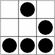
\includegraphics[width=0.5cm]{img/logo_glider.png} }
\fancyfoot[RO]{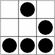
\includegraphics[width=0.5cm]{img/logo_glider.png} \hfill
	\MainTitle 
\hfill \thepage /\pageref{LastPage}}
\renewcommand{\headrulewidth}{0.25pt}
\renewcommand{\footrulewidth}{0.50pt}
\addtolength{\headheight}{0.5pt}
\fancypagestyle{plain}{
	\fancyhead{}
	\renewcommand{\headrulewidth}{0pt}
}

%--- Definitions de nouvelles commandes ---
\newcommand{\N}{\mathbb{N}} % les entiers naturels

%--- Definitions de nouvelles couleurs ---
\definecolor{verylightgrey}{rgb}{0.8,0.8,0.8}
\definecolor{verylightgray}{gray}{0.80}
\definecolor{lightgrey}{rgb}{0.6,0.6,0.6}
\definecolor{lightgray}{gray}{0.6}

%============================= Corps =================================
\begin{document}

\setlength\parindent{0pt}

%% \texttt{  }~\\

%% \textbf{\LARGE }~\\

%% \emph{\small }~\\

%% \begin{minipage}[ht]{0.75\textwidth}
%% 	~\\
%% \end{minipage} \hfill \begin{minipage}[ht]{6.15cm}
%% 	\includegraphics[width=6.00cm]{img/*****}
%% \end{minipage}~\\~\\

%% \clearpage

%% \section*{Bibliography\markboth{Bibliography}{Bibliography}}
%% \addcontentsline{toc}{section}{Bibliography}
%% \bibliography{bibliography} %% .bib
%% \bibliographystyle{frplain} % plain or frplain

\texttt{http://www.rue89.com/2013/11/15/dark-net-mythologie-vient-247532}~\\

\textbf{<< Darknet >>, cet autre Internet appel{\'e} {\`a} un bel avenir de mythologie terrifiante}~\\

\emph{\small Arr{\^e}t sur images --- 15/11/2013 {\`a} 10h32 --- Daniel Schneidermann -- Fondateur d'@rr{\^e}t sur images  }~\\

Comment l'appeler ? << Deep Net >> ? << Darknet >> ? Internet profond ? Une chose est s{\^u}re, cet << autre >> Internet, cette zone de non-droit, que \texttt{d{\'e}peignait jeudi soir << Envoy{\'e} sp{\'e}cial >>~\footnote{\texttt{http://www.france2.fr/emissions/envoye-special/videos/91829800}}} dans un reportage saisissant, est appel{\'e} {\`a} un bel avenir de mythologie terrifiante. Attendez-vous, dans les semaines qui viennent, aux couvertures d'hebdos alarmantes, et aux {\'e}loquentes interpellations {\`a} l'Assembl{\'e}e. ~\\

Sombre, profond : oubliez toutes vos r{\'e}f{\'e}rences terrestres, nous sommes ici dans les catacombes, dans les tunnels des conspirateurs, 20 000 lieues sous les mers, dans le monde du silence de Cousteau. ~\\

\textbf{Quatre jours pour recevoir son P38} ~\\

Comme dans les catacombes, on n'y acc{\`e}de que par un logiciel, TOR, qui permet au visiteur de surfer en toute tranquillit{\'e}, rigoureusement intra\c{c}able, sans laisser nulle part son adresse IP. Comble de la stup{\'e}faction : cet espace << {\'e}chappe aux moteurs de recherche >>. Oui, on peut y {\'e}chapper aux avenues {\'e}clair{\'e}es et balis{\'e}es par Google, et {\`a} la surveillance de tous les inquisiteurs du Web, pour y batifoler dans un labyrinthe de ruelles sombres, coupe-gorge, cour des miracles, o{\`u} \texttt{le Bitcoin a supplant{\'e} le dollar~\footnote{\texttt{http://www.arretsurimages.net/chroniques/2013-04-18/Bitcoin-invention-geniale-ou-arnaque-id5777}}}. ~\\

Comme dans toute terra incognita digne de ce nom, se c{\^o}toient le pire et le meilleur, soigneusement renvoy{\'e}s dos {\`a} dos par l'enqu{\^e}teur de France 2, dans un balancement fascination-r{\'e}pulsion qui ressuscite brutalement les mythologies de l'apparition d'Internet, {\`a} la fin du si{\`e}cle dernier, quand Daniel Bilalian nous terrifiait avec le monstre ambivalent. ~\\

\textbf{The Silk Road, march{\'e} noir de la drogue} ~\\

Les sites de vente d'armes (efficaces : << Envoy{\'e} sp{\'e}cial >> a re\c{c}u en quatre jours le \texttt{P38~\footnote{\texttt{http://fr.wikipedia.org/wiki/Walther\_P38}}} command{\'e}) y c{\^o}toient les h{\'e}ro{\"i}ques reporters charg{\'e}s de couvrir l'Afghanistan. Reporters sans fronti{\`e}res organise {\`a} Kaboul des stages de formation {\`a} TOR pour journalistes. Les amateurs de sites p{\'e}dophiles y fr{\^o}leront sans le savoir les r{\'e}sistants {\`a} l'espionnage de la NSA. C'est dans ce Dark Net, que se trouve Silk road, ce magasin en ligne de vente de drogues, \texttt{terrass{\'e} par le FBI~\footnote{\texttt{http://www.arretsurimages.net/breves/2013-10-04/Drogue-bitcoin-la-presse-s-alarme-Un-peu-vite-id16174}}} le mois dernier, et \texttt{qui vient de rena{\^i}tre~\footnote{\texttt{http://www.arretsurimages.net/breves/2013-11-14/Silk-Road-le-site-de-nouveau-accessible-id16414}}} de ses ruines. ~\\

Vrai ? Faux ? Quelle part de r{\'e}alit{\'e}, quelle part de boursouflure journalistique habituelle ? Impossible de le discerner a priori. Les grandes cha{\^i}nes de t{\'e}l{\'e}vision, depuis quinze ans, nous ont tellement -- et France 2 au premier rang -- habitu{\'e}s {\`a} la diabolisation d'Internet, ses p{\'e}dophiles en libert{\'e}, ses marchands d'armes, ses garages {\`a} bombes artisanales, qu'il est d{\'e}sormais difficile de les croire sur le sujet, m{\^e}me quand par hypoth{\`e}se elles diraient vrai. Ce qui ouvre un champ prometteur aux enqu{\^e}tes ind{\'e}pendantes. ~\\

\clearpage

\texttt{http://www.telerama.fr/medias/darknet-immersion-en-reseaux-troubles,102055.php}~\\

\textbf{Darknet : immersion en r{\'e}seaux troubles}~\\

\emph{\small Le 14/09/2013 {\`a} 00h00 -- Olivier Tesquet -- T{\'e}l{\'e}rama n\degre 3322 }~\\

\begin{minipage}[ht]{9.25cm}
	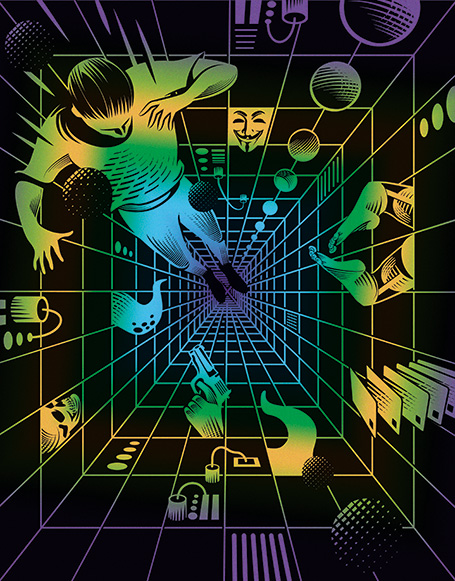
\includegraphics[width=9.00cm]{img/darknet-immersion-en-reseaux-troubles,M124676.jpg}~\\
	\emph{Illustration : Yann Legendre pour T{\'e}l{\'e}rama }~\\
\end{minipage} \hfill \begin{minipage}[ht]{10.00cm}
	\textbf{\textsc{Enqu{\^e}te} | Monde parall{\`e}le aux contours infinis, ce Web bis anonyme o{\`u} le pire c{\^o}toie le meilleur nourrit tous les fantasmes. Bienvenue dans le Darknet. }~\\

	Depuis Galil{\'e}e, on sait que la Terre est ronde. Mais Internet ? On le sait prot{\'e}iforme, on l'imagine infini. On conna{\^i}t moins son ultime fronti{\`e}re, son dernier p{\'e}age avant le n{\'e}ant ou, plut{\^o}t, le grand n'importe quoi : une zone non cartographi{\'e}e, hors de port{\'e}e des radars, et qu'on appelle commun{\'e}ment le <<Darknet>>. ~\\

	Sombre et clandestin, inconnu du grand public, c'est un royaume de l'anonymat, inaccessible depuis un navigateur traditionnel. Sa r{\'e}putation est sulfureuse, et il y r{\'e}gnerait une ambiance proche de celle des bas-fonds de \emph{Blade Runner~\footnotemark}. P{\^e}le-m{\^e}le, il mettrait la p{\'e}do-pornographie {\`a} port{\'e}e de souris, offrirait aux polytoxicomanes de tous les pays un hypermarch{\'e} o{\`u} faire leurs courses et proposerait {\`a} prix cass{\'e} des num{\'e}ros de carte Bleue par palettes enti{\`e}res. Il a m{\^e}me ses l{\'e}gendes urbaines, comme ces combats {\`a} mort de gladiateurs modernes retransmis par webcam (mais que personne n'a jamais vus). ~\\
\end{minipage}~\\
\footnotetext{\texttt{http://www.telerama.fr/tag/blade-runner/}}

\textbf{\large Un corps invert{\'e}br{\'e}}~\\

L'animal se conjugue au pluriel. La vie y est moins manich{\'e}enne que dans un reportage d'\emph{Enqu{\^e}te exclusive} : le pire c{\^o}toie souvent le meilleur, sans panneaux indicatifs. Difficile {\`a} cerner, impossible {\`a} mesurer, le Darknet est un corps invert{\'e}br{\'e}. Que les initi{\'e}s parcourent avec discr{\'e}tion. Les dinosaures du Web, sous pr{\'e}texte de ne pas susciter de mauvaises vocations, r{\'e}pugnent {\`a} le faire conna{\^i}tre. Le Darknet, c'est un peu comme la premi{\`e}re r{\`e}gle du Fight Club dans le roman de Chuck Palahniuk : on n'en parle pas. Sauf quand il surgit, par erreur, par effraction, dans la vie civilis{\'e}e. ~\\

C'est ce qui est arriv{\'e}, au mois d'avril, {\`a} la faveur du ph{\'e}nom{\`e}ne \texttt{bitcoin~\footnote{\texttt{http://www.telerama.fr/medias/bitcoins-le-cash-du-siecle,102056.php}}}. Dans les m{\'e}dias, tout {\`a} coup, le quidam a appris qu'un krach venait de se produire, celui d'une monnaie virtuelle, internationale, d{\'e}centralis{\'e}e et anonyme. Une monnaie marginale, hors de tout contr{\^o}le. ~\\

Les m{\'e}dias ont profit{\'e} de l'actualit{\'e} pour sortir leur double d{\'e}cim{\`e}tre, tenter de jauger l'insondable profondeur de cette terra (presque) incognita. France Inter a {\'e}voqu{\'e} <<\emph{un Internet parall{\`e}le sans limite ni protection}>> ; Marianne, dissert{\'e} sur un <<\emph{monde interlope}>> dans lequel il faudrait plonger t{\^e}te la premi{\`e}re. Arpenter le Darknet, c'est immanquablement convoquer l'image de l'apn{\'e}iste qui descend dans l'abysse, fermement accroch{\'e} {\`a} sa gueuse. Et d{\'e}velopper tous les fantasmes. Qu'en est-il r{\'e}ellement ? ~\\


\begin{minipage}[ht]{0.40\textwidth}
	\textbf{\large Difficile {\`a} capturer}~\\

	D'abord, le Darknet ne doit pas {\^e}tre confondu avec le <<Deep Web>>, le Web profond, qui regroupe les sites accessibles librement mais non index{\'e}s par les moteurs de recherche. Selon une {\'e}tude publi{\'e}e en 2001, ce dernier, traditionnellement repr{\'e}sent{\'e} comme la partie immerg{\'e}e d'un iceberg, ferait plus de cinq cents fois la taille du Web commercial. Le Darknet, lui, si tant est qu'on puisse le nommer ainsi, est encore plus difficile {\`a} capturer. ~\\
\end{minipage} \hfill \colorbox{verylightgray}{%
	\begin{minipage}{0.50\textwidth}
		\footnotesize
		\textbf{\large Satoshi Nakamoto, le p{\`e}re du bitcoin}~\\

		La question br{\^u}le les l{\`e}vres des journalistes depuis de longs mois : qui se cache derri{\`e}re ce myst{\'e}rieux alias japonisant ? Le cr{\'e}ateur du bitcoin, c'est la seule certitude. Mais existe-t-il ? Surgi de nulle part en 2008 (impossible de trouver une trace de son existence avant la cr{\'e}ation du bitcoin), l'homme de l'ombre pourrait n'{\^e}tre qu'une couverture. ~\\

		Une enqu{\^e}te du New Yorker est remont{\'e}e jusqu'{\`a} Michael Clear, un {\'e}tudiant du prestigieux Trinity College de Dublin. Mais au moins une douzaine d'autres noms ont {\'e}t{\'e} avanc{\'e}s. De quoi alimenter les th{\'e}ories les plus fantaisistes. En attendant, Nakamoto reste invisible, comme la <<main>> d'Adam Smith. %% ~\\
	\end{minipage}%
} \hfill ~\\

Comme l'explique Okhin, un jeune trentenaire qui se d{\'e}finit avec provocation comme un <<\emph{cryptoterroriste}>>, <<\emph{un darknet est un r{\'e}seau qui n'est pas connect{\'e} {\`a} Internet. Chacun d'entre eux est une maison, et il faut la bonne cl{\'e} pour y p{\'e}n{\'e}trer}>>. Il en existe donc des myriades, corps autonomes reli{\'e}s entre eux par des passerelles aux noms barbares, comme \texttt{I2P~\footnote{\texttt{http://www.i2p2.de/}}} (Invisible Internet Project) ou \texttt{TOR~\footnote{\texttt{https://www.torproject.org/}}}. ~\\

TOR, c'est justement le moyen le plus simple de passer la t{\^e}te par l'entreb{\^a}illement de cet Internet qui n'en est pas un. Acronyme de <<The Onion Router>>, le routeur en oignon, TOR a d'abord {\'e}t{\'e} con\c{c}u {\`a} des fins militaires avant de devenir le dernier rempart de milliers d'activistes qui ont le malheur de vivre sous des horizons peu cl{\'e}ments pour la libert{\'e} d'expression. Par extension, il s'est {\'e}galement impos{\'e} comme le meilleur alli{\'e} de tous ceux qui ont quelque chose {\`a} cacher. ~\\

Son principe est redoutable : lorsqu'un internaute se connecte au r{\'e}seau, ses paquets de donn{\'e}es transitent {\`a} travers plusieurs couches (d'o{\`u} la m{\'e}taphore de l'oignon), ce qui a pour objectif de dissimuler son identit{\'e}. Ainsi, en quelques heures sur le Darknet, mon adresse IP [la plaque d'immatriculation de mon ordinateur, ndlr] s'est tour {\`a} tour promen{\'e}e entre les serveurs de l'h{\'e}bergeur \texttt{OVH~\footnote{\texttt{http://www.ovh.com/fr/index.xml}}} {\`a} Roubaix, le relais d'un informaticien de l'Ontario... et le prestigieux Massachusetts Institute of Technology (\texttt{MIT~\footnote{\texttt{http://www.telerama.fr/idees/le-mit-une-bulle-de-savants,88591.php}}}). ~\\

	\textbf{\large Le grand bazar du Wiki cach{\'e}}~\\

	Une fois parachut{\'e}s en territoire inconnu, oubliez les familiers .fr ou .com. Sur TOR, nous sommes tous des marins d'eau douce en .onion. Pour les explorateurs qui ne conna{\^i}traient pas leur destination finale, \texttt{The Hidden Wiki~\footnotemark } (le <<Wiki cach{\'e}>>) offre un rapide panorama des ressources du Darknet. Ce portail, qui ressemble {\`a} s'y m{\'e}prendre {\`a} Wikip{\'e}dia, recense certaines des adresses les plus populaires. Dans ce bazar mal {\'e}tiquet{\'e}, on trouve des <<services financiers et commerciaux>> aussi divers que des comptes Paypal d{\'e}j{\`a} approvisionn{\'e}s ou des faux papiers, ainsi que des revendeurs {\`a} la sauvette de produits Apple qui promettent de reverser <<\emph{15 \% de leurs b{\'e}n{\'e}fices {\`a} des orphelinats}>>. ~\\

	Outre une vaste offre de solutions d'h{\'e}bergement et de courriel, le Wiki cach{\'e} liste aussi bien des blogs parodiques sur la derni{\`e}re campagne pr{\'e}sidentielle am{\'e}ricaine que des forums consacr{\'e}s {\`a} l'occultisme ou {\`a} la fabrication d'armes {\`a} feu {\`a} l'aide d'imprimantes 3D. Au milieu d'un annuaire pornographique poliment nomm{\'e} Erotica, on trouve m{\^e}me l'int{\'e}grale des \emph{Spirou Magazine}. Au d{\'e}tour d'une page, un lien pointe vers \texttt{The Silk Road~\footnotemark }, litt{\'e}ralement <<la route de la soie>>, un Amazon de la drogue qui permet d'acheter toutes sortes de compos{\'e}s chimiques interdits par la loi. Ici, chaque acheteur {\'e}value le vendeur, la qualit{\'e} de la marchandise, les d{\'e}lais de livraison. Un v{\'e}ritable site d'e-commerce o{\`u} toutes les transactions se r{\`e}glent... en bitcoins. ~\\
\footnotetext{\texttt{http://www.thehiddenwiki.net/}}
\footnotetext{\texttt{http://www.thehiddenwiki.net/silk-road-what-it-is-how-to-access-it/}}

\begin{minipage}[ht]{7.25cm}
	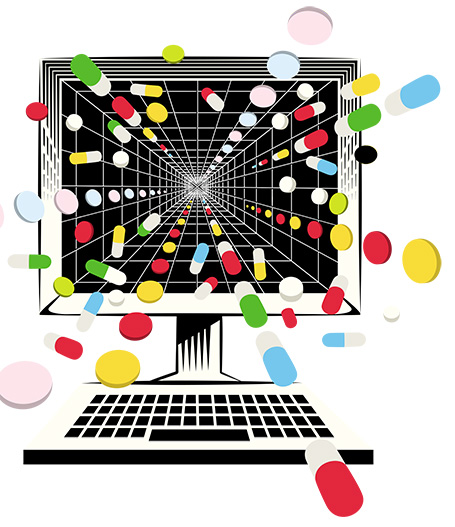
\includegraphics[width=7.00cm]{img/darknet-immersion-en-reseaux-troubles,M124681.jpg}~\\
	\emph{Illustration : Yann Legendre pour T{\'e}l{\'e}rama }~\\
\end{minipage} \hfill \begin{minipage}[ht]{12.00cm}
	A l'heure du \texttt{scandale Prism~\footnotemark }, r{\'e}v{\'e}l{\'e} par \texttt{Edward Snowden~\footnotemark }, le Darknet est aussi la base arri{\`e}re des d{\'e}fenseurs des libert{\'e}s individuelles, notamment ceux qui combattent la surveillance des r{\'e}seaux par l'Etat, par Google, par Facebook. On y retrouve toute la panoplie de l'<<hacktiviste>> sensible {\`a} la protection des libert{\'e}s num{\'e}riques : un onglet <<Political advocacy \& whistleblowing>> (activisme politique et lanceurs d'alerte), des sites miroirs de WikiLeaks, un reliquat d'\texttt{Indymedia~\footnotemark } (qui fut au d{\'e}but des ann{\'e}es 2000 le lieu de rassemblement virtuel des alter-mondialistes). ~\\
	
	\textbf{\large Au rayon des bidouilleurs}~\\

	On croise les bidouilleurs au grand complet : les phreakers, capables de pirater les lignes t{\'e}l{\'e}phoniques ; les crackers, dont le passe-temps pr{\'e}f{\'e}r{\'e} consiste {\`a} s'introduire sur des sites auxquels ils ne sont pas cens{\'e}s acc{\'e}der ; ou encore la communaut{\'e} <<warez>>, qui s'est fait un devoir de diffuser librement du contenu en th{\'e}orie prot{\'e}g{\'e} par la propri{\'e}t{\'e} intellectuelle. Certains petits malins, moins bien intentionn{\'e}s que d'autres, proposent des services de location de botnets (un parc de machines zombies) pour mener des attaques par d{\'e}ni de service (une attaque qui consiste {\`a} saturer un site de requ{\^e}tes, le mode d'action pr{\'e}f{\'e}r{\'e} des \texttt{Anonymous~\footnotemark }). ~\\
\end{minipage}~\\
\footnotetext{\texttt{http://www.telerama.fr/medias/scandale-prism-nouvelles-revelations-sur-un-programme-d-espionnage-visant-l-ue,99654.php}}
\footnotetext{\texttt{http://www.telerama.fr/personnalite/edward-snowden,510291.php?xtatc=INT-41}}
\footnotetext{\texttt{http://www.indymedia.com/}}
\footnotetext{\texttt{http://www.telerama.fr/tag/anonymous/}}

Vous pouvez {\'e}galement adresser des dons aux partis pirates, {\`a} l'\texttt{Internet Archive~\footnotemark } (une association am{\'e}ricaine qui joue le r{\^o}le d'une biblioth{\`e}que d'Alexandrie num{\'e}rique), ou encore {\`a} \texttt{WikiLeaks~\footnotemark }. Soumis {\`a} un blocus financier de Visa et de MasterCard fin 2011, le site de Julian Assange avait trouv{\'e} la parade en se mettant {\`a} accepter les dons... en bitcoins. --- Pr{\'e}cis{\'e}ment, le Darknet est le refuge des cryptoanarchistes, qu'Okhin d{\'e}finit en une formule. <<\emph{La cryptoanarchie est une {\'e}quation math{\'e}matique selon laquelle il est impossible d'{\'e}couter les communications si elles sont chiffr{\'e}es dans leur ensemble}>>, explique-t-il d'un ton docte, casquette de la \texttt{NSA~\footnotemark } - l'agence de s{\'e}curit{\'e} nationale am{\'e}ricaine - viss{\'e}e sur le cr{\^a}ne. ~\\
\footnotetext{\texttt{http://archive.org/index.php}}
\footnotetext{\texttt{http://wikileaks.org/}}
\footnotetext{\texttt{http://www.telerama.fr/medias/qui-la-nsa-peut-elle-traquer-a-peu-pres-tout-le-monde,98909.php}}

\colorbox{verylightgray}{%
	\begin{minipage}{0.475\textwidth}
		\footnotesize
		\textbf{\large Phil Zimmermann, le cryptographe}~\\

		Sa notori{\'e}t{\'e}, Phil Zimmermann la doit {\`a} une proc{\'e}dure judiciaire kafka{\"i}enne. En 1991, il met {\`a} disposition du public un logiciel de chiffrement : \texttt{PGP~\footnotemark }, pour Pretty Good Privacy. D{\'e}sormais, tout un chacun peut communiquer de mani{\`e}re confidentielle, bien abrit{\'e} derri{\`e}re une technologie militaire. ~\\

		Mais les autorit{\'e}s am{\'e}ricaines go{\^u}tent peu l'initiative. La cryptographie {\'e}tant consid{\'e}r{\'e}e comme une arme, les douanes vont passer trois ans {\`a} essayer de faire tomber Zimmermann pour une violation imaginaire de la loi sur l'exportation. Aujourd'hui chef d'entreprise, il est consid{\'e}r{\'e} comme l'un des p{\`e}res fondateurs de la s{\'e}curit{\'e} informatique. Et, par extension, du Darknet. %% ~\\
	\end{minipage}%
} \hfill \colorbox{verylightgray}{%
	\begin{minipage}{0.475\textwidth}
		\footnotesize
		\textbf{\large Ian Clarke, parrain du Darknet}~\\
		
		Au d{\'e}part, tout pr{\'e}destinait cet Irlandais de 36 ans {\`a} venir gonfler les rangs des soldats de la Silicon Valley. C'est d'ailleurs le chemin qu'il avait d{\'e}cid{\'e} d'emprunter, d{\'e}m{\'e}nageant {\`a} la fin des ann{\'e}es 90 pour la Californie apr{\`e}s des {\'e}tudes d'informatique {\`a} l'universit{\'e} d'Edimbourg. ~\\
		
		Et s'il n'a pas compl{\`e}tement abandonn{\'e} cette voie (il vit aujourd'hui {\`a} Austin, Texas, et dirige une poign{\'e}e de start-up), l'histoire se souviendra de lui comme le cr{\'e}ateur de Freenet, pionnier des r{\'e}seaux peer-to-peer d{\'e}centralis{\'e}s. %% ~\\
	\end{minipage}%
} ~\\
\footnotetext{\texttt{http://www.siteduzero.com/informatique/tutoriels/la-cryptographie-facile-avec-pgp}}

En choisissant de dispara{\^i}tre du Web marchand, les anars du code choisissent en quelque sorte de br{\^u}ler leur carte d'identit{\'e}. Ils fuient la centralisation, la g{\'e}olocalisation, la publicit{\'e} cibl{\'e}e, le tra\c{c}age de leurs donn{\'e}es personnelles ou de leurs historiques de navigation. <<\emph{Aujourd'hui, les Etats gouvernent par le secret, alors que tout ce que nous faisons en ligne devient public, peste Okhin. Nous tentons d'inverser cette polarit{\'e}.}>> Maquisards des temps ultramodernes, les <<alternautes>> dans son genre militent pour le droit d'<<\emph{{\^e}tre seuls avec }[eux-m{\^e}mes]>> sans {\^e}tre suivis {\`a} la trace dans leurs d{\'e}placements en ligne. ~\\

Dans leur esprit, le Darknet, les darknets, leurs darknets, sont l'utopie r{\'e}alis{\'e}e des Zones autonomes temporaires (ZAT) d'Hakim Bey~\footnotemark , <<\emph{{\^i}les en r{\'e}seau}>> ou <<\emph{enclaves libres}>> {\'e}chappant {\`a} toute tentative de d{\'e}finition. Parfois, ils arrivent m{\^e}me {\`a} trouver des ramifications jusque dans le monde r{\'e}el, comme {\`a} Notre-Dame-des-Landes, o{\`u} des mini-r{\'e}seaux autonomes ont germ{\'e}, outils d'organisation invisibles de la ZAD, devenue <<\emph{zone {\`a} d{\'e}fendre}>>. ~\\
\footnotetext{Hakim Bey : \emph{De son vrai nom Peter Lamborn Wilson, le po{\`e}te am{\'e}ricain doit sa notori{\'e}t{\'e} {\`a} une pens{\'e}e anarchiste orthodoxe, particuli{\`e}rement populaire dans les sous-cultures libertaires du Web.}}

\begin{minipage}[ht]{7.25cm}
	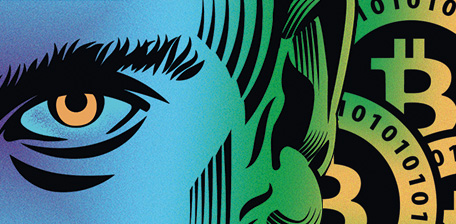
\includegraphics[width=7.00cm]{img/darknet-immersion-en-reseaux-troubles,M124682.jpg}~\\
	\emph{Illustration : Yann Legendre pour T{\'e}l{\'e}rama }~\\
\end{minipage} \hfill \begin{minipage}[ht]{12.00cm}
	\textbf{\large La libert{\'e} d'expression et ses limites}~\\

	Confront{\'e} {\`a} des questions voltairiennes, rousseauistes, centenaires, de limites {\`a} la libert{\'e} d'expression, le Darknet porte au revers de son veston la vieille maxime de Benjamin Franklin : <<\emph{Un peuple pr{\^e}t {\`a} sacrifier un peu de libert{\'e} pour un peu de s{\'e}curit{\'e} ne m{\'e}rite ni l'une ni l'autre.}>> Alors, est-il intrins{\`e}quement bon, subsidiairement mauvais ? Ou peut-{\^e}tre l'inverse, tant il refuse de choisir son camp. La r{\'e}ponse, partiale, discutable, pol{\'e}mique, pourrait venir de Ian Clarke. ~\\
\end{minipage}~\\

Cet ing{\'e}nieur irlandais a d{\'e}velopp{\'e} \texttt{Freenet~\footnotemark }, un r{\'e}seau dans le r{\'e}seau qui se pr{\'e}sente sous la forme d'un logiciel install{\'e} sur votre ordinateur. Revendiquant pr{\`e}s de trente mille membres actifs (c'est-{\`a}-dire que leur machine est un <<nœud>>, un point d'intersection du r{\'e}seau), \texttt{il expliquait son point de vue radical au Guardian en 2009~\footnotemark } : ~\\
\footnotetext{\texttt{https://freenetproject.org/?language=fr}}
\footnotetext{\texttt{http://www.theguardian.com/technology/2009/nov/26/dark-side-internet-freenet}}

<<\emph{La pornograpie infantile existe sur Freenet, mais elle existe partout sur Internet. Nous pourrions {\'e}laborer un virus pour l'{\'e}radiquer, c'est techniquement possible. Mais nous commencerions rapidement {\`a} recevoir des injonctions concernant par exemple la propri{\'e}t{\'e} intellectuelle. Nous serions somm{\'e}s de supprimer tout contenu suspect. Modifier Freenet signerait la fin de Freenet.}>> Tol{\'e}rer l'intol{\'e}rable au nom de la sauvegarde de la libert{\'e} d'expression, voil{\`a} le d{\'e}fi qu'impose le Darknet. Vous {\^e}tes pr{\'e}venus. ~\\ 

\dotfill %% \clearpage

\texttt{http://rue89.nouvelobs.com/2014/02/03/internet-linsecurite-existe-ca-nest-si-grave-249585}~\\

\textbf{Sur Internet, l'ins{\'e}curit{\'e} existe et \c{c}a n'est pas (si) grave}~\\

\emph{\small Ce qui nous arrive sur la Toile 03/02/2014 {\`a} 10h31 -- Xavier de La Porte | France Culture }~\\

L'ins{\'e}curit{\'e} existe aussi sur Internet : hier soir encore, on apprenait que les donn{\'e}es personnelles de 800 000 clients d'Orange avaient {\'e}t{\'e} pirat{\'e}es, une menace qui p{\`e}se sur toute entreprise poss{\'e}dant des donn{\'e}es sensibles (on pense aux banques en particulier). --- Sur Internet, on peut se faire arnaquer (par exemple, envoyer 500 euros {\`a} un ami prof de fran\c{c}ais qui est coinc{\'e} {\`a} l'{\'e}tranger et vous a envoy{\'e} un mail plein de fautes d'orthographe). Sur les r{\'e}seaux sociaux, les jeunes peuvent se faire harceler, les vieux le d{\'e}sirent mais \c{c}a ne leur arrive pas. Parfois, c'est un virus qui arrive d'on ne sait o{\`u} et qui met {\`a} bas notre ordinateur. ~\\

Sur ce qu'on appelle le <<Darknet>> (une sorte d'espace assez fantasmatique qui r{\'e}unit les sites non index{\'e}s sur le web, des r{\'e}seaux anonymis{\'e}s), on trouve des contenus p{\'e}dophiles, on peut acheter des armes, de la drogue... --- Je pourrais prolonger cette {\'e}num{\'e}ration ad nauseam. Bref, l'ins{\'e}curit{\'e} num{\'e}rique existe et elle alimente un {\'e}norme march{\'e}, celui de la s{\'e}curit{\'e} informatique, qui vise {\`a} prot{\'e}ger techniquement les entreprises, institutions et particuliers contre ces d{\'e}sagr{\'e}ments. ~\\

\textbf{\large Cyber-harc{\`e}lement et poubelle connect{\'e}e}~\\

L'ins{\'e}curit{\'e} num{\'e}rique se double d'un sentiment d'ins{\'e}curit{\'e} qui s'impose au m{\'e}pris de toute proportion, de toute distinction entre les formes de dangers, dans un processus que l'on conna{\^i}t bien par ailleurs. ~\\

On m{\'e}lange la question des failles techniques avec les mauvaises intentions, on m{\'e}lange l'envie de ne pas {\^e}tre surveill{\'e} (l'anonymat) avec des activit{\'e}s ill{\'e}gales - m{\'e}lange symptomatique dans la mani{\`e}re dont on aborde le fameux <<Darknet>> -, on prend des cas tr{\`e}s rares (par exemple les cas o{\`u} le cyber-harc{\`e}lement de jeunes gens a eu des cons{\'e}quences tragiques) comme les embl{\`e}mes de d{\'e}rives massives. ~\\

Ce sentiment d'ins{\'e}curit{\'e} aliment{\'e} par nous, les m{\'e}dias. Par exemple, j'ai toujours {\'e}t{\'e} fascin{\'e} par la mani{\`e}re dont un journal t{\'e}l{\'e}vis{\'e} pouvait traiter {\`a} quelques minutes de distance le cyber-harc{\`e}lement des adolescents sur Facebook (c'est horrible, terrifiant), puis les derni{\`e}res innovations dans un salon technologique quelconque (la poubelle connect{\'e}e, c'est g{\'e}nial...). ~\\

Le tout sans jamais faire le lien entre les deux, ou m{\^e}me expliquer que l'impression d'ins{\'e}curit{\'e} num{\'e}rique croit {\`a} mesure que le num{\'e}rique prend dans nos vies - et dans l'{\'e}conomie - une part une plus importante. ~\\

Qu'est-ce que produit ce sentiment d'ins{\'e}curit{\'e} ? Qu'est-ce que produit ce m{\'e}lange des dangers ? Eh bien, des tentatives de politiques s{\'e}curitaires. ~\\

\textbf{\large L'acc{\`e}s {\`a} Internet reconnu comme un droit}~\\

Dans le champ du num{\'e}rique, cela prend une forme particuli{\`e}re : la tentation des gouvernements successifs {\`a} d{\'e}l{\'e}guer l'application des lois {\`a} des autorit{\'e}s administratives. ~\\

Pour le dire autrement, la s{\'e}curit{\'e} num{\'e}rique ne rel{\`e}verait pas de la justice, mais d'un droit d{\'e}rogatoire, o{\`u} des autorit{\'e}s administratives ind{\'e}pendantes pourraient :
\begin{itemize}
	\item \textbf{filtrer} les contenus ;
	\item en \textbf{bloquer} certains ;
	\item faire \textbf{fermer} des sites ;
	\item \textbf{priver} des particuliers de leur acc{\`e}s {\`a} Internet...
\end{itemize}

Tout cela sans passer devant un juge, sans proc{\'e}dure contradictoire. ~\\

Symbole de cette tentation : en 2011, {\'e}tait lanc{\'e}e par un ancien ministre UMP l'id{\'e}e de cr{\'e}er une Haute autorit{\'e} du Net qui, pour lutter contre les escroqueries, le t{\'e}l{\'e}chargement ill{\'e}gal, la p{\'e}dophilie ou m{\^e}me l'incitation {\`a} la haine, aurait eu le pouvoir de fermer un site sans aucune proc{\'e}dure judiciaire. ~\\

Folie direz-vous. Je vous rappelle qu'{\`a} l'origine, l'Hadopi, c'{\'e}tait cela, appliqu{\'e} au respect du droit d'auteur. On pouvait apr{\`e}s quelques avertissements priver quelqu'un s'{\'e}tant livr{\'e} au t{\'e}l{\'e}chargement ill{\'e}gal de l'acc{\`e}s {\`a} Internet - acc{\`e}s consid{\'e}r{\'e} comme un droit par l'ONU - et cela sans que la Justice n'ait rien {\`a} dire. ~\\

Dans les faits, et gr{\^a}ce {\`a} des mobilisations fortes, l'HADOPI n'a jamais pris ces mesures. Mais la tentation est grande et ne se limite pas aux gouvernements de droite. ~\\

\textbf{\large Un droit {\`a} part pour nos vies num{\'e}riques}~\\

Tout derni{\`e}rement, un article du projet de loi pour l'{\'e}galit{\'e} homme-femme s'inscrivait encore dans cette logique, il a {\'e}t{\'e} vot{\'e} au S{\'e}nat, puis retir{\'e}. Et l'id{\'e}e du gouvernement consistant {\`a} transf{\'e}rer les objectifs et comp{\'e}tences de l'HADOPI au CSA (le Conseil Sup{\'e}rieur de l'Audiovisuel, une autre autorit{\'e} administrative donc) n'est pas compl{\`e}tement {\'e}trang{\`e}re {\`a} tout cela. ~\\

Vous me direz que ce n'est pas tr{\`e}s grave, que dans une d{\'e}mocratie, on n'a rien {\`a} craindre d'une autorit{\'e} administrative ind{\'e}pendante. Peut-{\^e}tre. ~\\

Ce qu'on {\`a} craindre, me semble-t-il, c'est d'accepter que nos vies num{\'e}riques soient soumises {\`a} un r{\'e}gime de droit {\`a} part, comme si, parce que c'est technique, parce que c'est compliqu{\'e}, le pouvoir politique pouvait se passer de la justice en ces mati{\`e}res. Ce n'est jamais bon quand le pouvoir politique pense pouvoir se passer de la justice. ~\\


\end{document}
